\subsection{分层状态机与任务转换}
\subsubsection{状态机的层次建模与实际控制入口}
最新路线程序没有用一个枚举变量表达所有状态，而是由 Route 线程、phase 索引、循环分支及 go/\texttt{stop\_\allowbreak ev} 事件共同实现。报告将其抽象为三层：任务层管理 A/B/C 目标次序，单段层根据观测选择对中、直行或等待，执行层串行播放动作帧。图中的状态名称用于解释控制流，不意味着源码存在同名类。状态机描述因此必须同时交代进入条件、动作和退出事件。

任务层的 ROUTE 列表为 A-left、B-right、C-stop。每进入一段，steps、turns、misses、blind、progress、\texttt{last\_\allowbreak seen} 等局部记录重置，避免上一段观测影响下一目标。corner 成功返回后才推进 phase；阶段切换不是仅靠固定时间或预设转向次数。抓取播放结束建立锁臂值，但最新入口没有同时检查颜色持物证据，不能把动作结束写成传感器已确认抓住。
\begin{figure}[H]\centering\begin{tikzpicture}[
state/.style={draw=Navy!65,line width=.8pt,rounded corners=3pt,fill=Navy!3,text width=38mm,minimum height=21mm,align=center,inner sep=3mm,font=\small,text=black},
action/.style={state,draw=Teal,fill=Teal!6},
edge/.style={-{Stealth[length=2.3mm]},line width=.9pt,draw=Navy},
trigger/.style={font=\footnotesize,text=Navy,fill=white,inner sep=1.4pt}]
\node[state] (s) at (0,0) {\textbf{01\quad 等待启动}\\[1.5mm]按 S／自动延时};
\node[action] (g) at (5.5,0) {\textbf{02\quad 抱起并锁臂}\\[1.5mm]\texttt{grab\_final\_v2}};
\node[state] (a) at (11,0) {\textbf{03\quad 走向 A}\\[1.5mm]观测、对中、前进};
\node[action] (l) at (11,-3) {\textbf{04\quad 左转寻找 B}\\[1.5mm]最多 12 次尝试};
\node[state] (b) at (5.5,-3) {\textbf{05\quad 走向 B}\\[1.5mm]重置单段运行计数};
\node[action] (r) at (0,-3) {\textbf{06\quad 右转寻找 C}\\[1.5mm]确认下一目标可见};
\node[state] (c) at (0,-6) {\textbf{07\quad 走向 C}\\[1.5mm]持续观测终点目标};
\node[action] (p) at (5.5,-6) {\textbf{08\quad 解锁并放置}\\[1.5mm]\texttt{put\_down}};
\node[state] (d) at (11,-6) {\textbf{09\quad 结束任务}\\[1.5mm]退出线程、保留日志};
\draw[edge] (s)--node[trigger,above] {启动}(g);
\draw[edge] (g)--node[trigger,above,align=center] {动作\\完成}(a);
\draw[edge] (a)--node[trigger,right] {到达 A}(l);
\draw[edge] (l)--node[trigger,above] {看到 B}(b);
\draw[edge] (b)--node[trigger,above] {到达 B}(r);
\draw[edge] (r)--node[trigger,right] {看到 C}(c);
\draw[edge] (c)--node[trigger,above] {到达 C}(p);
\draw[edge] (p)--node[trigger,above,align=center] {动作\\完成}(d);
\end{tikzpicture}
\caption{最新 marker\_route 任务主状态转换。到达条件来自距离或近距丢码启发式，转角成功要求下一目标可见。}\label{fig:hum-main-fsm}\end{figure}

主状态图表达的是阶段顺序，而每个“走向”状态内部还包含反复观测与动作选择。阶段切换有两个不同守卫：抵近当前目标触发固定方向的转角搜索；确认下一目标可见后才推进路线索引。这样的划分使转角失败可以保留当前阶段，避免一次丢码就跳过目标。

\source{\code{humanoid/maze_route/marker_route.py}：Route.\_run、corner、ROUTE。}

\subsubsection{初始化、启动和锁臂状态}
启动先建立日志目录，解析参数及图形模式，再构造 Servos、固定头部、打开 Eyes、启动 Route 线程。真实舵机模式尝试关闭占用串口的厂家程序并停止服务；这是资源准备，不是机器人路线的一部分。交互模式等待 S 设置 go，无头模式在 \texttt{start\_\allowbreak delay} 后启动。no-grab 跳过初始抱起，但仍从 \texttt{grab\_\allowbreak final\_\allowbreak v2} 尾帧读取锁臂值，因此假定物块和机械姿态已经就位。

六个身体通道固定为抓取末帧，其他通道由步态决定。锁臂约束保护命令中的抱持姿态，不测量夹持力。若末帧来源与实际抓取动作不一致，即使下肢轨迹不变，也可能在起步时改变手臂。最新程序用自己的 actions 副本，不应混入旧 grab 文件的尾帧数值。
\begin{equation}
\mathcal A=\{6,7,8,14,15,16\},\qquad p_{k,i}=\begin{cases}p_{\mathrm{last},i}^{\mathrm{grab}},&i\in\mathcal A,\\p_{k,i}^{\mathrm{gait}},&i\notin\mathcal A.\end{cases}
\end{equation}
运行开关的含义及其任务前提汇总如下，目的是区分离线检查、已抱物起步和完整搬运流程。
\begin{table}[H]\centering\small\begin{tabularx}{\linewidth}{p{30mm}Y}\toprule 模式 & 实际含义\\\midrule
dry-run & Route.act 不走转，但仍可能打开串口并设置头部\\
no-servos & 不触碰舵机串口，隐含 dry-run\\
no-grab & 已抱物起步假设，仍读取抓取尾帧用于锁臂\\
no-release & 到 C 停止但不放置，不符合完整放置任务\\\bottomrule\end{tabularx}\caption{运行模式与任务前提。}\end{table}

这些开关改变的是执行条件和任务完整性，并非同一功能的等价测试方式。特别是禁用舵机的离线检查不能验证抓取可靠性，而跳过放置的运行也不能计为完整搬运成功。

\source{\code{marker_route.py}：main、Servos、Route.act。}

\subsubsection{三阶段目标与距离守卫}
A/B/C 既是模板 ID，也是路线语义。A 是第一段末端，抵近后左转寻找 B；B 是第二段末端，抵近后右转寻找 C；C 是终点，抵近后停止与放置。程序只统计当前 target 的观测，其他码即使同时出现，也不自动跳过当前阶段。距离阈值在前两段使用 \texttt{turn\_\allowbreak cm}，在末段使用 \texttt{stop\_\allowbreak cm}，默认都是 40 cm。

这里的距离是相机到码中心的三维斜距，不是机器人几何中心到围挡的地面净距。码的高度、相机偏置、脚步余程和身体外包络都会影响安全停车位置。报告应记录码安装与实际摆位，不将“阈值40 cm”解释为所有机体部分与障碍都有40 cm余量。看到下一码是转角结束条件，但不能证明精确完成90度；后续对中仍会改变朝向。
\begin{equation}
(A,\mathrm{left})\rightarrow(B,\mathrm{right})\rightarrow(C,\mathrm{stop}),\qquad d_{A,B}\le d_{\mathrm{turn}},\quad d_C\le d_{\mathrm{stop}}.
\end{equation}
\source{\code{marker_route.py}：ROUTE、limit、phase 与 corner 调用。}

\subsection{固定标记识别与视觉测距}
\subsubsection{自定义标记的编码与透视解码}
标记由9乘9格组成，外两格为黑边，中间5乘5数据。markers.py 保存三张25位模板，并在四个旋转方向寻找最少数据位差异；最多允许1格数据错误，黑边最多允许3格读白。图\ref{fig:hum-patterns}直接读取实际模板常量，不是新生成的替代码，也不是标准ALVAR、ArUco或AprilTag字典。

检测先对灰度图高斯滤波、自适应二值化并寻找轮廓，要求凸四边形和足够的最短边像素；过度拉伸的候选被排除。透视展开到固定网格后，采样每格内部，降低边缘插值和印刷边界影响，再按Otsu阈值分类黑白。若内外轮廓重复命中同一码，优先采用数据错误更少、边长更大的候选。识别依赖真实黑边完整、像素大小和成像质量，允许一位误读并不等于对大面积遮挡鲁棒。
\begin{figure}[H]\centering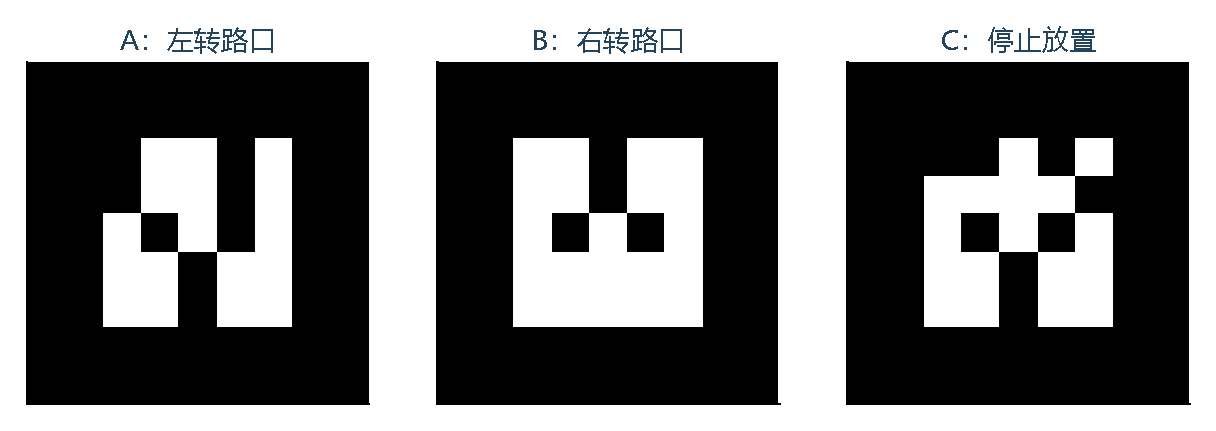
\includegraphics[width=.9\linewidth]{figures/analysis/marker_patterns.pdf}\caption{源码中实际 A/B/C 数据模板及其路线含义，黑色正方形边长设计值为14 cm。}\label{fig:hum-patterns}\end{figure}

三种图案把视觉身份绑定为不同路线语义，识别出 A、B、C 后仍需结合当前阶段决定是否采用。黑边与内部数据共同参与解码，打印尺寸则进入后续测距模型。模板图主要用于核对目标设计，识别容错还要通过旋转后的数据位距离分析。

\source{\code{humanoid/maze_route/markers.py}：TEMPLATES、\_read、MarkerDetector.detect。}

\subsubsection{模板旋转分离度与尺寸一致性}
设数据位串为a和b，Hamming距离统计不同格子的数量。四旋转中的最小差异反映有限字典的分离程度；对角线为零，非对角项应足够大，才有识别容错余量。图中的矩阵由真实模板直接计算，不能当作实机识别混淆矩阵，也不提供误识别概率。
\begin{equation}
d_{\mathrm H}(a,b)=\sum_{j=1}^{25}\mathbb1(a_j\ne b_j),\qquad d^*_{ab}=\min_{r\in\{0,1,2,3\}}d_{\mathrm H}(a,\operatorname{rot}_{90r}(b)).
\end{equation}
模板旋转rot与相机解算的目标方位、墙面朝向是不同输出，rot=90不能解释成机器人转了90度。增大打印尺寸能提高远端像素支持，却同时改变近端出画面条件。若实际边长变了而\texttt{SIZE\_\allowbreak CM}仍为14，PnP将产生尺度偏差；新增模板也必须重新检查所有旋转的距离，而不仅观察正立图案是否不同。
\begin{figure}[H]\centering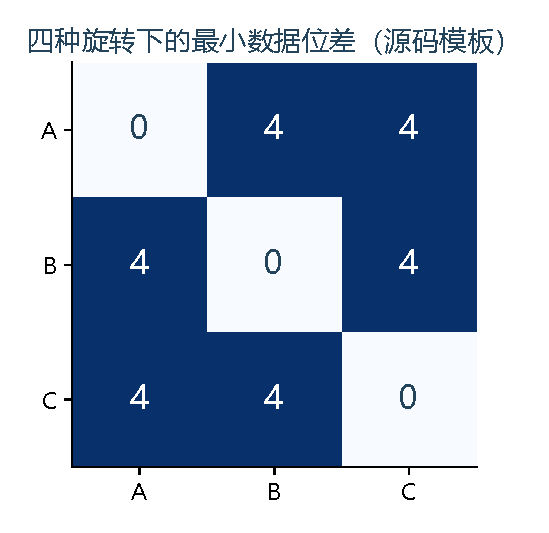
\includegraphics[width=.64\linewidth]{figures/analysis/hamming.pdf}\caption{实际模板在四旋转下的最小数据位差，不是性能测试。}\end{figure}

矩阵应按非对角元素解读：数值越大，两个不同模板在最相似旋转下仍有越多格不同。该结构性质支持设置有限的数据位容错，但未包含模糊、反光和角点提取误差，因此不能直接推算现场识别成功率。后续距离估计仍依赖几何标定的一致性。

\source{\code{markers.py}：SIZE\_CM、\_ROT、MAX\_DATA\_ERR。}

\subsubsection{PnP 距离、方位和墙面姿态}
检测器用已知正方形四角、设备标定内参和畸变参数，通过\texttt{SOLVEPNP\_\allowbreak IPPE\_\allowbreak SQUARE}求旋转和平移。\texttt{dist\_\allowbreak cm}取平移向量范数；\texttt{bearing\_\allowbreak deg}由去畸变后的标记中心横坐标求反正切；墙面yaw则由标记法向推导。三者量纲和含义不同，路线对中主要使用bearing，不能因为模块输出yaw就宣称采用了完整位姿控制。
\begin{equation}
\lambda\tilde u=K[R\mid t]\tilde X,\quad d=\|t\|_2,\quad \beta=\arctan(u_n),\quad d=\sqrt{d_h^2+\Delta h^2}.
\end{equation}
码与镜头存在高度差时，斜距大于水平距离。距离误差还受打印尺寸、角点、标定、运动模糊和观察角影响。下图右侧按水平40 cm绘制几何关系，不是设备测距精度。正式标定要用同一定义的真实斜距，或同时记录水平距离和高度差，避免把量纲不同的距离直接计算RMSE。
\begin{figure}[H]\centering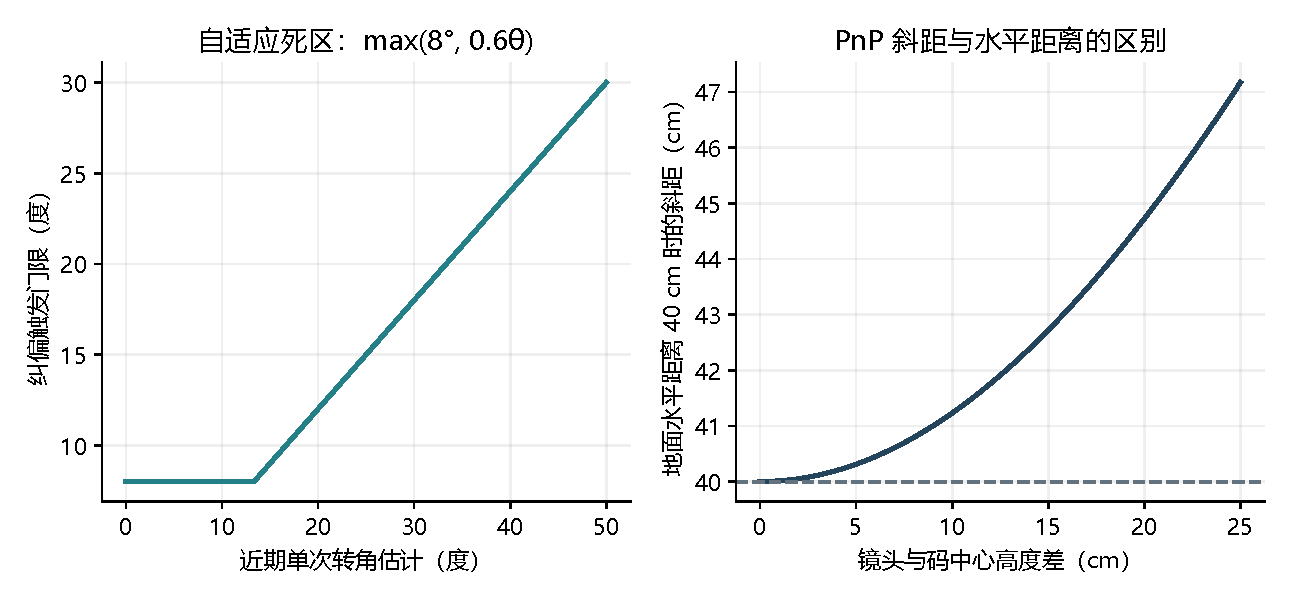
\includegraphics[width=\linewidth]{figures/analysis/control_geometry.pdf}\caption{纠偏门限解析曲线与斜距几何。两者为公式分析，非实测性能曲线。}\end{figure}

左图在近期转角估计较小时保留固定死区，超过交点后门限随估计线性增加；右图则表明，相同水平间距在高度差增大时产生更大的视觉斜距。两项分析分别影响是否纠偏和何时停车，调参时必须保持二者的物理含义独立，不能用调整纠偏门限补偿测距尺度误差。

\source{\code{markers.py}：MarkerDetector.\_measure；\code{marker_route.py}：CALIB。}

\subsection{单段决策、纠偏与转角控制}
\subsubsection{新帧、多数可见与单段观测状态}
Eyes线程持续更新frame、found和seq。look开始时记录seq0，只接受序号增加的新帧，默认观察3帧。凑不齐新帧返回no-camera；取得3帧但目标仅出现0或1帧返回None；至少2帧看见才对距离、方位分别取中位数。seen字段是可见帧数与新帧数之比，不是神经网络置信度。

中位数减少单帧抖动，却不能校正系统性标定错误。序号增长避免缓存图重复累计，但图像是否真正近期仍依赖\texttt{robust\_\allowbreak camera}的取流契约。动作结束后还有0.25 s稳态等待，再开始新的look，防止直接用大幅身体运动期间画面作下一步判断。

有新帧但无目标与相机断流进入不同分支。相机断流原地等待；目标无效则可能受限盲行和补偿。图\ref{fig:hum-leg-fsm}保留这个区别，避免把“所有失锁均停车”写成当前源码已实现行为。
\begin{figure}[H]\centering\begin{tikzpicture}[
box/.style={draw=Navy!65,line width=.8pt,rounded corners=3pt,fill=Navy!3,text width=32mm,minimum height=15mm,align=center,inner sep=2.5mm,font=\small,text=black},
act/.style={box,draw=Teal,fill=Teal!6},
warn/.style={box,draw=Rust,fill=Rust!6},
judge/.style={diamond,aspect=2.3,draw=Navy,line width=.8pt,fill=white,text width=27mm,inner sep=1.5mm,align=center,font=\small,text=black},
edge/.style={-{Stealth[length=2.2mm]},draw=Navy,line width=.85pt},
tag/.style={font=\footnotesize,fill=white,inner sep=1.2pt,text=Navy}]
\node[box] (obs) at (0,0) {\textbf{稳态观测}\\获取 3 个新帧、取中位数};
\node[warn] (cam) at (4.7,0) {\textbf{相机无新帧}\\原地等待；超时暂停或退出};
\node[judge] (valid) at (0,-2.4) {\textbf{目标有效？}};
\node[warn] (blind) at (-4.7,-2.4) {\textbf{目标不可见}\\受限盲行与偏航补偿\\超限则暂停／退出};
\node[judge] (arr) at (0,-4.8) {\textbf{满足到达条件？}};
\node[act] (next) at (4.7,-4.8) {\textbf{结束当前路段}\\进入转角或终点放置};
\node[judge] (err) at (0,-7.2) {\textbf{方位误差超限？}\\$|\beta|>\tau$};
\node[act] (walk) at (-2.8,-9.6) {\textbf{直行一步}\\更新推进与偏航记录};
\node[act] (turn) at (2.8,-9.6) {\textbf{执行一次纠偏}\\重新观测转角效果};
\draw[edge] (obs)--node[tag,above] {无新帧}(cam);
\draw[edge] (obs)--node[tag,right] {有新帧}(valid);
\draw[edge] (valid)--node[tag,above] {否}(blind);
\draw[edge] (valid)--node[tag,right] {是}(arr);
\draw[edge] (arr)--node[tag,above] {是}(next);
\draw[edge] (arr)--node[tag,right] {否}(err);
\draw[edge] (err.west)-|node[tag,pos=.25,above] {容差内}(walk.north);
\draw[edge] (err.east)-|node[tag,pos=.25,above] {偏差大}(turn.north);
\draw[edge] (blind.south)--(-4.7,-8.6)-|node[tag,pos=.25,left,align=center] {未超\\限制}(walk.west);
\draw[draw=Teal,line width=.8pt] (walk.south)--(-2.8,-10.8)--(2.8,-10.8)--(turn.south);
\draw[edge,draw=Teal] (0,-10.8)--(0,-11.3)--(-7.2,-11.3)--(-7.2,0)--(obs.west);
\node[tag,text=Teal] at (-3.6,-11.3) {动作完成、稳态等待后再次观测};
\end{tikzpicture}
\caption{单段观测—决策—动作状态。动作完成后回到获取新帧，盲行分支受计数约束。}\label{fig:hum-leg-fsm}\end{figure}

该图强调判断顺序：先区分相机断流与目标丢失，再检查到达条件，最后决定纠偏或直行。相机无新帧不产生新的前进指令；有画面但无目标则进入受计数限制的分支。底部回路说明动作结束后必须重新观测，上一轮方位不能连续驱动多步。近距丢码的到达推断与盲行补偿细则见后文。

\source{\code{marker_route.py}：Eyes.look、Route.\_run。}

\subsubsection{多帧投票如何改变动作入口}
图\ref{fig:vote-analysis}枚举三个新帧中目标可见的全部八种组合，用于解释\code{Eyes.look}的判据。只有至少两帧可见时才采用距离与方位的中位数；在三个新帧尚未收齐时，程序进入相机等待，而不把缺帧填成“未见目标”。
\begin{figure}[H]\centering
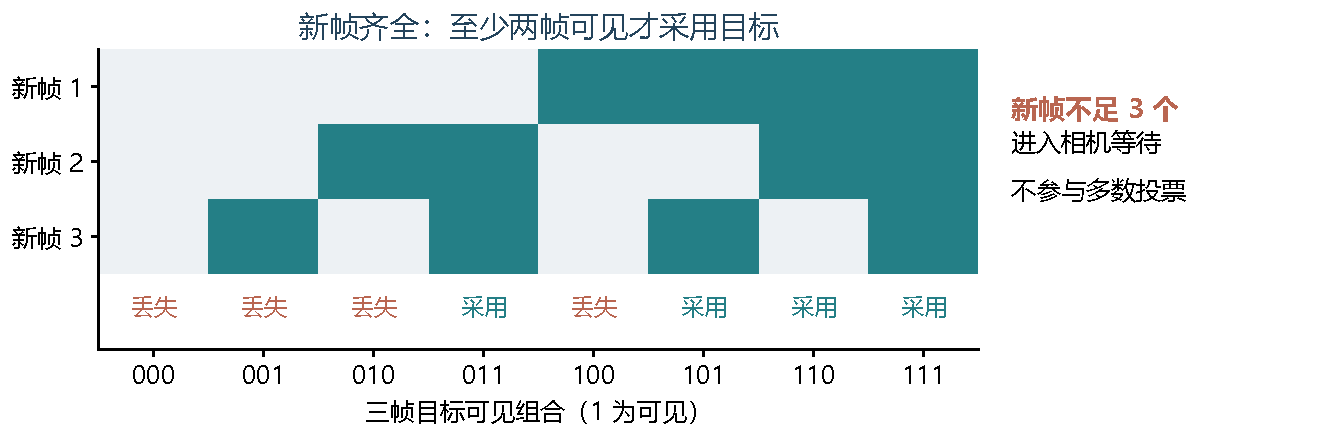
\includegraphics[width=.95\linewidth,height=.25\textheight,keepaspectratio]{figures/enriched/observation_vote.pdf}
\caption{三个新帧的多数可见判据。此图为源码条件穷举，不是识别准确率或概率分布。}\label{fig:vote-analysis}
\end{figure}
八种组合并不等概率，连续帧的模糊与遮挡还可能高度相关，因此不能从“八种中四种采用”推出50\%成功率。中位数能降低偶发异常对一次决策的影响，却不能修正错误标定或持续误识别。现场记录应把“缺帧”“足帧但不可见”“多数可见且采用”分别编码，才能辨别等待来自取流链还是标记检测。
\source{\code{marker_route.py}：Eyes.look。}

\subsubsection{自适应纠偏、转角学习与离散振荡}
双足转向动作一次可能产生较大角度。误差只有几度就转一次，会让目标跨到画面另一侧，导致来回纠偏。程序使用近期五个有效转角效果的中位数，并把门限设为\texttt{centre\_\allowbreak deg}与其60\%的较大值；默认\texttt{centre\_\allowbreak deg}为8度，初始\texttt{turn\_\allowbreak step\_\allowbreak deg}为20度。
\begin{equation}
\hat\theta=\operatorname{median}(\Theta_{t-4:t}),\qquad |\beta|>\max(8^\circ,0.6\hat\theta).
\end{equation}
转向后重新观测当前码，以方位变化绝对值更新估计，仅接收3至60度之间的变化。这个估计受到身体平移、码位置和角点噪声影响，不是IMU纯航向测量。为把流程图中的判断落实到数值空间，图\ref{fig:decision-region}假设近期单次转角为30度，因此门限18度，只在有效观测条件下绘制。容差内继续前进是效率与偏差的折中，连续纠偏次数过多仍会暂停，不应从实验记录中删除这类失败事件。
决策区域图给出了前述流程在有效观测条件下的几何切片：斜距不超过 40 cm 时优先判定到达；尚未到达时，以正负 18 度分隔直行与纠偏区域。这里 18 度来自假设转角估计的 60\%，不是固定通用参数。该图不覆盖相机断流、计数超限或近距丢码分支，因而需要与流程图结合阅读。
\begin{figure}[H]\centering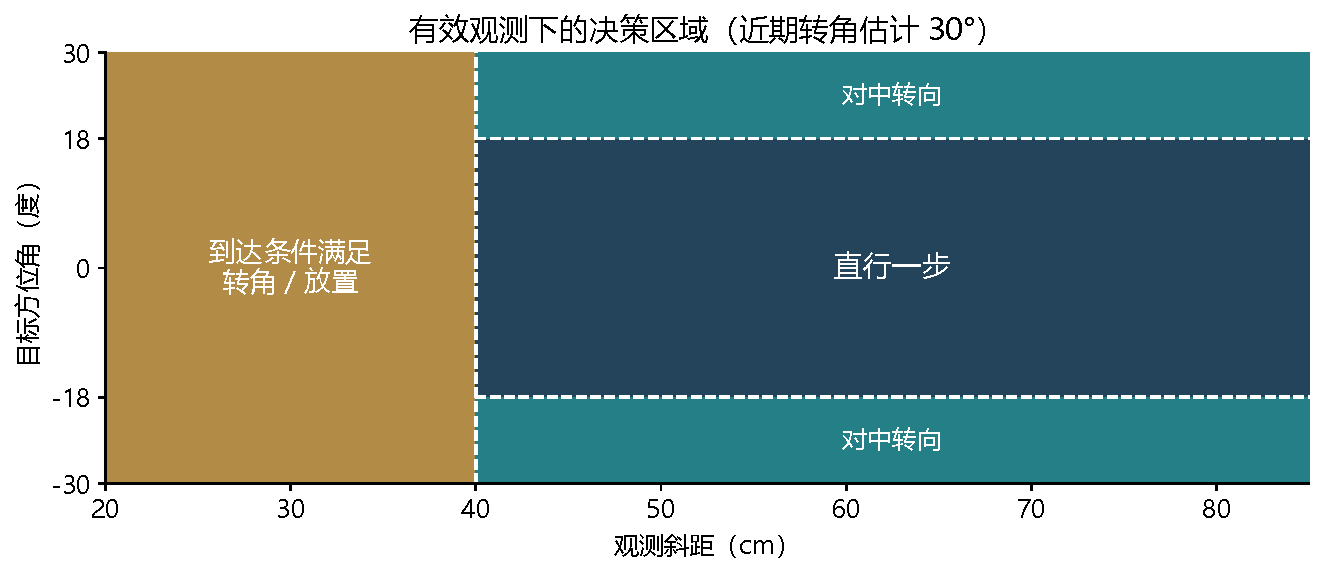
\includegraphics[width=.93\linewidth]{figures/analysis/decision_region.pdf}\caption{有效目标观测下的解析决策域：假设近期转角估计30度。}\label{fig:decision-region}\end{figure}

因此，日志中的距离变化与方位变化应先按当前阶段分开，再判断动作是否符合优先级。图中到达区不再按方位分割，正是“先到达、后纠偏”的程序分支顺序所致；不能把它读成到达时方位必然已居中。

\source{\code{marker_route.py}：turn\_steps、need、max\_centre\_turns。}

\subsubsection{直行偏航学习和受限盲行分支}
直行前后目标均可见且方位绝对值小于15度时，程序把前后方位差加入drift。至少三个样本后，可用近期15项中位数累计creep，在无目标时超过单次转角的60\%则纠偏。该量是图像方位的启发式变化，不是独立身体航向，也不是足端里程计；目标深度和相机晃动仍会影响估计。

首次未见目标和见过后丢失采用不同计数约束，\texttt{max\_\allowbreak misses}默认2，\texttt{max\_\allowbreak blind\_\allowbreak steps}默认25，另有每段步数上限。这一策略可能帮助远处C暂不可见时推进，却不能保证遮挡空间安全，且与课程失去目标后原地重捕获的严格要求存在差距。报告据实呈现分支；如果现场最终收紧策略，应绑定新的提交和参数再评价，而不是提前写成当前程序能力。
\begin{equation}
\hat\delta=\operatorname{median}(\Delta\beta_{t-14:t}),\qquad c_{k+1}=c_k+\hat\delta,\quad |c_k|>0.6\hat\theta\Rightarrow\text{反向纠偏}.
\end{equation}
\source{\code{marker_route.py}：prev\_walk\_obs、drift、blind、creep。}

\subsubsection{转角子状态机及最大尝试次数}
corner接收side和下一目标nxt。每次先停0.3 s，转一次，经act的0.25 s稳态等待，再停0.3 s观察下一码。成功返回只要求下一码有效可见，之后由下一段主循环继续对中；不是在corner里完成精准航向闭环。单周期耗时还包括文件动作时长、观测等待和SDK调用，不能只累加d6a时长估计全程。

若相机无新帧，corner原地等画面，不继续转动。默认最多12次转向，未见下一码则pause：有窗口等待S，再重试一轮；无头模式退出。恢复保留任务阶段，但姿态已经变化，应核对目标与场地，不能把S恢复描述成回到最初起点重跑。
\begin{figure}[H]\centering\begin{tikzpicture}[box/.style={draw=Navy!65,line width=.8pt,rounded corners=3pt,fill=Navy!3,text width=35mm,minimum height=19mm,align=center,inner sep=3mm,font=\small,text=black},act/.style={box,draw=Teal,fill=Teal!6},warn/.style={box,draw=Rust,fill=Rust!6},edge/.style={-{Stealth[length=2.3mm]},line width=.9pt,draw=Navy},tag/.style={font=\footnotesize,text=Navy,fill=white,inner sep=1.3pt}]
\node[box] (a) at (0,0) {\textbf{确定搜索方向}\\[1mm]A 后左转／B 后右转};
\node[act] (t) at (5.3,0) {\textbf{执行一次转向}\\[1mm]等待、转向、稳态等待};
\node[box] (v) at (10.6,0) {\textbf{观测下一标记}\\[1mm]检查 B 或 C 是否可见};
\node[act] (ok) at (10.6,-3) {\textbf{下一标记可见}\\[1mm]返回主循环、继续对中};
\node[warn] (retry) at (5.3,-3) {\textbf{未见下一标记}\\[1mm]累计尝试；最多 12 次};
\node[warn] (fail) at (0,-3) {\textbf{搜索失败}\\[1mm]交互暂停／无头退出};
\draw[edge] (a)--node[tag,above] {进入转角}(t);
\draw[edge] (t)--node[tag,above] {动作完成}(v);
\draw[edge] (v)--node[tag,right] {可见}(ok);
\draw[edge] (v.south west)--node[tag,above,sloped] {不可见}(retry.north east);
\draw[edge] (retry)--node[tag,above] {达到上限}(fail);
\draw[edge] (retry.north)--node[tag,right] {仍可尝试}(t.south);
\node[draw=Navy!30,fill=Navy!2,rounded corners=2pt,text width=145mm,align=left,inner sep=3mm,font=\small] at (5.3,-5.3) {\textbf{观测约束：}无新帧时原地等待，不盲目继续转向；成功条件是下一标记可见，并非精确完成 $90^\circ$ 转角。};
\end{tikzpicture}
\caption{转角寻找下一码的状态转换及失败出口。}\end{figure}

转角控制将一次步态动作与一次目标检查串行执行，下一标记可见才允许返回主路线。尝试次数上限约束的是搜索过程，不能据此推算固定转角角度。相机断流时等待新帧，避免在没有观测依据的情况下继续累积转向。

\source{\code{marker_route.py}：Route.corner、pause。}

\subsubsection{近距丢码推断、停滞保护与任务结束}
近距离码可能从画面下缘离开。obs为空但\texttt{last\_\allowbreak seen}距离不大于limit+12 cm，且方位在max(\texttt{centre\_\allowbreak deg},15度)内时，程序构造\texttt{lost\_\allowbreak close}观测并把距离截到limit。这是启发式到达，不是新的实时测距；相近条件下的遮挡也可能被解释为抵近，因此日志要区分直接观测和推断到达。

推进守卫默认检查20步内距离缩短是否超过5 cm，另有每段150步上限。它检测“动作多但接近不足”，不直接判断碰墙、滑步或电机故障。C到达后解除锁臂并播放\texttt{put\_\allowbreak down}，动作完成即返回，最新入口没有接入颜色放置确认链。正式结果需由视频和物体状态核验补足，不能把程序线程结束直接等同于完整比赛成功。
\source{\code{marker_route.py}：arrived\_blind、progress、stall\_steps、stop分支。}

\subsection{动作执行、运行保护与日志}
\subsubsection{当前动作文件与首帧过渡的实证分析}
最新动作副本从\texttt{grab\_\allowbreak final\_\allowbreak v2}尾帧锁臂，六个刻度为566、908、40、435、108、935。下图实际读取最新actions目录，横轴帧号，纵轴身体通道，颜色为命令刻度。帧号不是等间隔时间；热图不代表编码器回传、力矩或接地状态，也不能从图中推断持物不掉落。

Servos.play比较首帧目标与上一命令pose：无已知姿态或任一身体通道差超过25刻度时，首帧至少延长到300 ms。pose初始化尝试读实际关节，后续通常是已发目标；并非每帧读反馈的动力学规划。放置动作解除锁臂，生成副本时首帧下蹲保持抱紧，后续松开与站起保持原设计。负载和地面变化仍需要受控实机验证。
\begin{figure}[H]\centering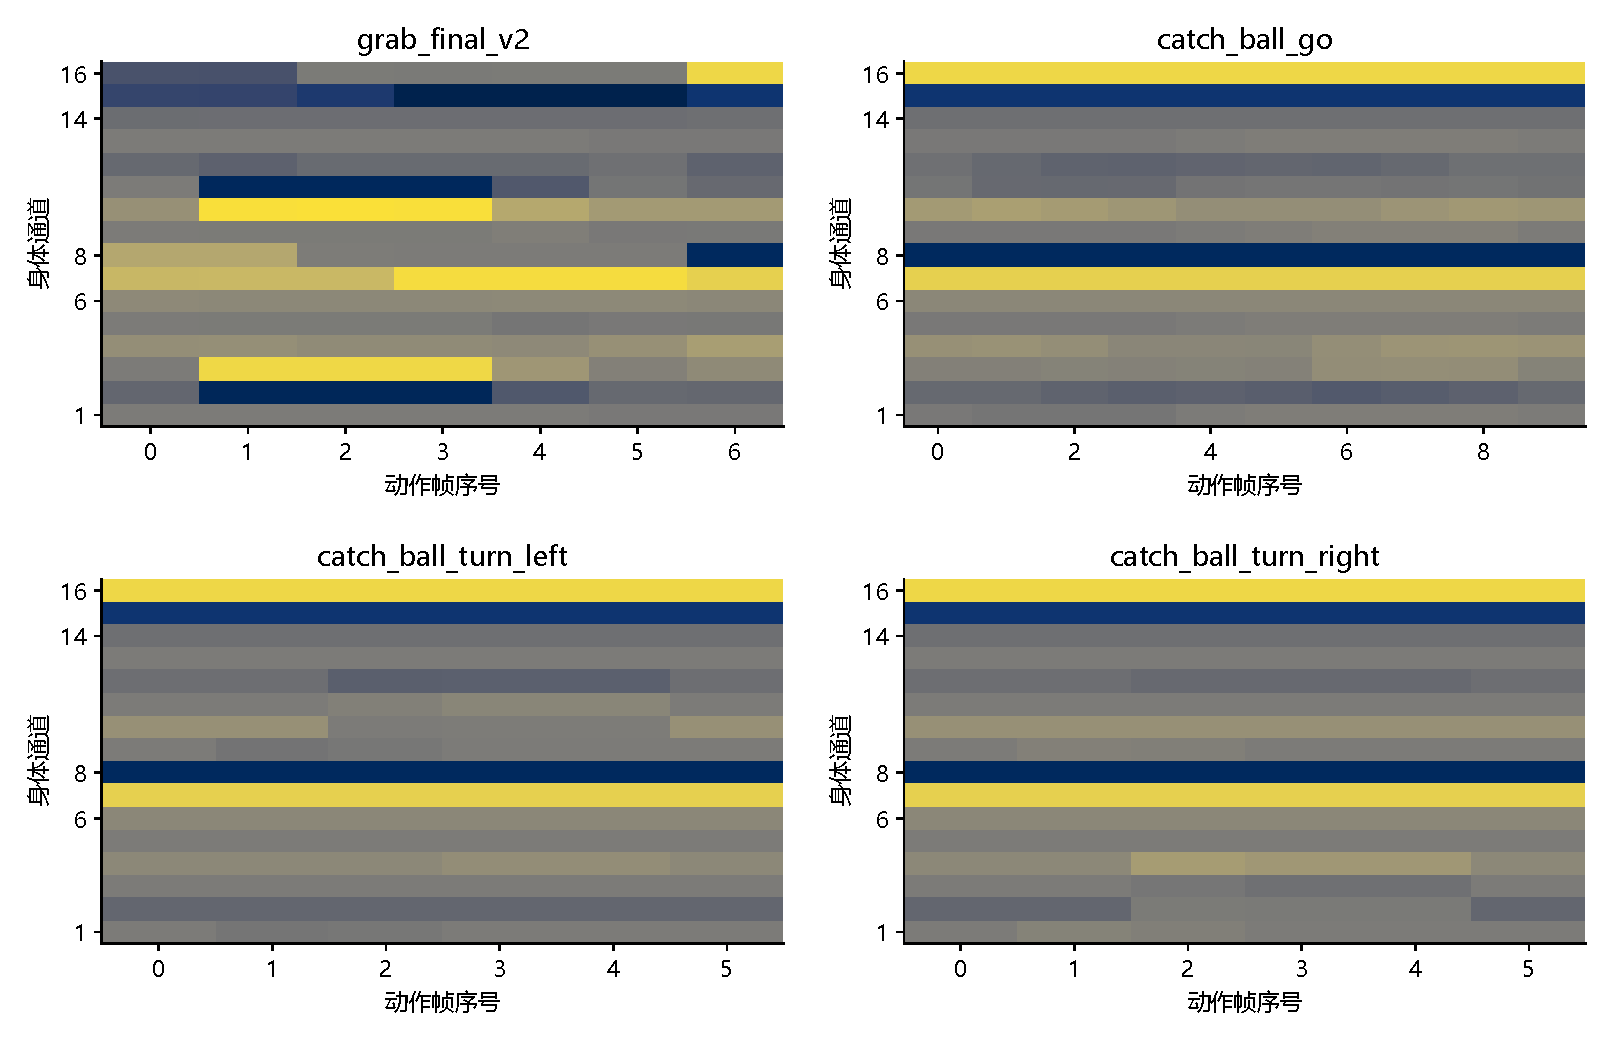
\includegraphics[width=\linewidth]{figures/analysis/current_actions.pdf}\caption{最新动作数据库的身体通道命令矩阵。数据源为真实动作文件，非仿真关节轨迹。}\end{figure}

热图中保持相同颜色的上肢通道用于核对锁臂约束，而下肢通道随动作帧变化形成步态。该表示可以发现动作副本是否意外改写抱持姿态，但无法证明实际关节已经到位。首帧过渡与负载下的运动连续性仍需结合动作时长和实机观察评价。

\source{\code{maze_route/actions}；\code{mkcopies.py}；\code{Servos.play}。}

\subsubsection{动作时间结构与闭环观测机会}
动作数据库提供了可直接计算的时序依据。图\ref{fig:action-budget}将每个动作的首帧与其余帧时长分开：抱起为9.50\,s，抱物直行为0.95\,s，左右转各1.00\,s，放置为7.10\,s。这里的数值仅为当前动作副本的帧时长之和，不包含额外等待、首帧延长和接口开销。
\begin{figure}[H]\centering
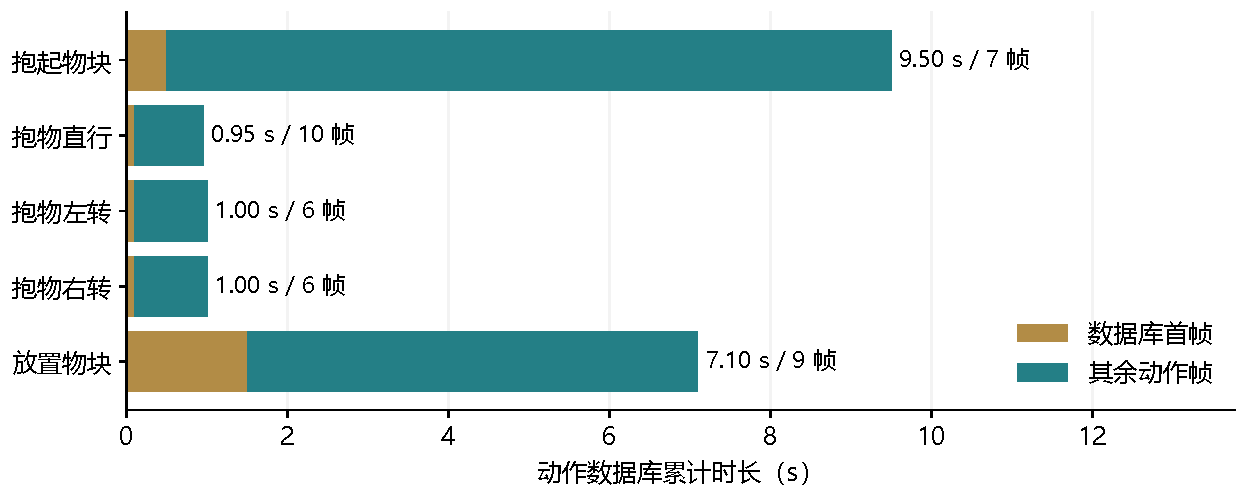
\includegraphics[width=.95\linewidth,height=.25\textheight,keepaspectratio]{figures/enriched/action_time_budget.pdf}
\caption{实际动作数据库的时长组成和帧数。条形长度表示文件内计划时间，非实测执行耗时。}\label{fig:action-budget}
\end{figure}
动作时间结构解释了为什么提高相机帧率不一定同比提高控制更新频率：路线线程通常先等一个完整动作返回，再稳态等待并重新观测。单次直行0.95\,s已构成明显的动作占用区间；若首帧因姿态差异被延长到至少0.30\,s，实际区间还会增加。对抓放这类较长动作，状态转换应依据播放完成与物理确认分别记录，而非只按墙钟定时跳转。

这一结构也提示优化的取舍。缩短动作可能增加纠偏机会，但会改变双足运动连续性与夹持稳定性；拆分动作以增加观测点，需要重新核对每个片段首尾姿态，而不能简单截掉动作帧。报告中的时间图据真实文件生成，为动作标定与异常日志对齐提供依据，不将计划时长当作机械性能结论。
\source{\code{humanoid/maze_route/actions/*.d6a}；\code{Servos.play}与\code{Route.act}。}

\subsubsection{交互暂停、无头退出与异常清理}
P清除go，控制后续动作是否获准执行，不撤回已发舵机帧；S重新设置go。Q/Esc或退出信号设置\texttt{stop\_\allowbreak ev}并置go，使等待线程得以退出，执行器在下一帧边界停止继续下发。软件停止后续帧与物理立即停止不同，电机当前插值与负载惯性仍存在。

pause在交互模式等S，无头模式直接结束。摄像头超时、转角失败、纠偏次数过多都可触发，但恢复点由各循环上下文决定。Route.run捕获异常写日志、置crashed并关闭CSV；主循环finally关闭相机和窗口、等待线程。该生命周期管理不等于倾倒保护或硬件急停。
\begin{figure}[H]\centering\begin{tikzpicture}[box/.style={draw=Navy!65,line width=.8pt,rounded corners=3pt,fill=Navy!3,text width=35mm,minimum height=19mm,align=center,inner sep=3mm,font=\small,text=black},act/.style={box,draw=Teal,fill=Teal!6},warn/.style={box,draw=Rust,fill=Rust!6},edge/.style={-{Stealth[length=2.3mm]},line width=.9pt,draw=Navy},tag/.style={font=\footnotesize,text=Navy,fill=white,inner sep=1.3pt}]
\node[act] (run) at (0,0) {\textbf{运行中}\\[1mm]\texttt{go = set}};
\node[warn] (pause) at (6.5,0) {\textbf{交互暂停}\\[1mm]\texttt{go = clear}};
\node[box] (end) at (0,-3.2) {\textbf{终止与资源清理}\\[1mm]停止后续帧、关闭资源};
\node[warn] (exit) at (6.5,-3.2) {\textbf{无头模式失败}\\[1mm]\texttt{stop\_ev = set}};
\draw[edge] ([yshift=3mm]run.east)--node[tag,above] {P／失败守卫}([yshift=3mm]pause.west);
\draw[edge] ([yshift=-3mm]pause.west)--node[tag,below] {S 恢复}([yshift=-3mm]run.east);
\draw[edge] (run)--node[tag,left] {Q／信号／异常}(end);
\draw[edge] (run.south east)--node[tag,above,sloped] {失败且无窗口}(exit.north west);
\draw[edge] (exit)--node[tag,above] {退出}(end);
\end{tikzpicture}
\caption{运行、暂停、恢复与退出状态；全局故障不等于自动重置路线。}\end{figure}

暂停与退出具有不同的生命周期：暂停保留阶段并等待恢复，退出则终止后续动作与资源使用。恢复箭头并不重建机器人位姿，也不会重新执行整条路线；因此恢复前需要确认物块、朝向和当前标记。图中的软件守卫不能替代硬件急停。

\source{\code{marker_route.py}：pause、wait\_running、Servos.play、main。}

\subsubsection{逐次日志形成的状态证据链}
route.log记录参数、阶段、转角学习与暂停退出，decisions.csv逐次记录phase、target、seen、斜距、方位、yaw、action、note，snapshots保存对应标注图。分析应先按phase切分，再统计walk、纠偏、盲行、corner、pause和stop，并在转移附近回看图像。这能说明每个状态转换的观测依据，而非只展示最终画面。

本次没有归档完整实机decisions.csv，因此状态图来自源码，动作图来自真实数据库，参数曲线是解析演示。后续可从真实日志绘制距离和方位时间线、动作事件带、相机断流和近距推断标记。最后一张识别框截图不能证明全程无失锁，日志中动作完成也不能证明无掉落或碰撞；这两类事实要由视频或传感器补充。
\source{\code{marker_route.py}：record、setup\_logging、overlay。}
